\documentclass[preprint,review,12pt]{elsarticle}
\usepackage{amsmath,amssymb}
\usepackage{graphicx}
\usepackage{booktabs}
\usepackage{array}
\usepackage{multirow}
\usepackage{xcolor}
\usepackage{siunitx}
\usepackage{algorithm}
\usepackage{algpseudocode}
\usepackage{circuitikz}
\usetikzlibrary{arrows.meta,positioning,fit,calc}
\usepackage{rotating}
\usepackage{etoolbox}
\usepackage{comment}
\usepackage{hyperref}
\hypersetup{hidelinks}
\sisetup{group-separator={,}, group-minimum-digits=4}
\newcommand{\gainp}{GainP}
\newcommand{\hyp}[1]{#1}   % assumptions and hypothesized content
\newcommand{\LF}{\mathit{LF}}
\definecolor{wosnewcolor}{RGB}{0,0,0}
\newcommand{\wosnew}[1]{#1}   % WOS-46985 results with retuned hyperparameters (2026-11-10)
% single line spacing inside floats, also in the double-spaced review layout
\definecolor{artemcolor}{RGB}{0,0,0}
\newcommand{\artem}[1]{#1}
\AtBeginEnvironment{table}{\linespread{1}\selectfont}
\AtBeginEnvironment{sidewaystable}{\linespread{1}\selectfont}
\AtBeginEnvironment{figure}{\linespread{1}\selectfont}
\AtBeginEnvironment{algorithm}{\linespread{1}\selectfont}
\journal{Expert Systems with Applications}

\begin{document}
\begin{frontmatter}

\title{Fuzzy-Pattern Tsetlin Machine Inference on a Gain Cell Embedded DRAM Associative In-Memory Processor}

\author[ind]{Artem Hnilov}
\author[biu]{Alexander Fish}
\author[biu]{Leonid Yavits\corref{cor1}}
\ead{leonid.yavits@biu.ac.il}
\cortext[cor1]{Corresponding author.}
\affiliation[ind]{organization={Independent Researcher}, country={France}}
\affiliation[biu]{organization={EnICS Labs, Faculty of Engineering, Bar-Ilan University},
            city={Ramat Gan}, postcode={5290002}, country={Israel}}

\begin{abstract}
The Fuzzy-Pattern Tsetlin Machine (FPTM) lets a clause vote with a reduced score when some of its literals fail. \artem{With the accuracy-oriented hyperparameters and $15\times$ to $25\times$ fewer clauses per class, FPTM reaches the accuracy of the most accurate strict Tsetlin Machine (TM) model on ALeRCE and NSL-KDD.}
We study whether this advantage survives in-memory inference on \gainp{}, a gain cell embedded DRAM associative processor.
We map FPTM inference onto the \gainp{} compare and write primitives in a sample-stationary and a clause-stationary layout.
A functional simulator confirms that the in-array predictions match a software reference \wosnew{on all checked test samples}.
The hardware evaluation targets a new, not yet fabricated \gainp{} design in a commercial 7~nm FinFET process.
We train FPTM, strict ($\LF=1$) and vanilla TM models on WOS-46985 text, ALeRCE astronomical light curves and NSL-KDD intrusion records.
\wosnew{With accuracy-oriented hyperparameters,} \hyp{the energy per classification in the sample-stationary layout is 0.15 to 112~nJ, including the controller. This lies within the range of published TM ASICs and in-memory designs and below that of TM FPGA accelerators. Under a 1~W core-power bound, a single-thread CPU needs at least $63\times$ more energy.}
\wosnew{A fuzzy clause costs a bit-serial miss count, so FPTM energy follows its included literals. Energy-oriented hyperparameters cut it by $1.6\times$ to $25\times$. On NSL-KDD, FPTM models then reach the accuracy band of the best strict model at $13\times$ to $23\times$ less energy. On ALeRCE, FPTM gives the cheapest points. On WOS-46985, strict models stay cheaper.}
\end{abstract}

\begin{highlights}
\item Fuzzy-Pattern Tsetlin Machine inference mapped onto a GC-eDRAM associative processor
\item Two layouts: input samples in memory columns, or clauses stored as ternary patterns
\item Both mappings simulated bit-exactly, with costs modeled for a 7 nm process
\item A strict clause costs one search, while a fuzzy one needs a bit-serial miss count
\item \wosnew{On NSL-KDD, energy-tuned FPTM reaches strict accuracy at 13x less energy}
\end{highlights}

\begin{keyword}
Tsetlin machine \sep Fuzzy-Pattern Tsetlin Machine \sep interpretable classification \sep
associative in-memory processing \sep gain cell eDRAM \sep content addressable memory
\end{keyword}
\end{frontmatter}

\section{Introduction}\label{sec:intro}

The Tsetlin Machine (TM) learns classifiers as sets of conjunctive clauses over Boolean literals~\cite{granmo2018tsetlin}.
Its inference uses only AND, NOT and counting.
This makes the TM attractive for interpretable and energy-efficient edge inference.
Reported TM hardware includes digital designs~\cite{wheeldon2020learning}, FPGA accelerators~\cite{tunheim2025fpga} and in-memory computing with resistive and Y-Flash devices~\cite{ghazal2023imbue,ghazal2025impact}.
Model compression for edge TM inference has also been studied~\cite{maheshwari2023redress}.

Each TM clause is a propositional rule over Boolean feature conditions.
A trained TM is therefore a rule base that a domain expert can inspect.
This property matters in decision-support applications.
Rudin argues that high-stakes decisions should use interpretable models rather than explained black boxes~\cite{rudin2019stop}.
In network intrusion detection, operators need to understand what a detector reports before they can act on it~\cite{sommer2010outside}.
In time-domain astronomy, alert brokers such as ALeRCE classify the alert streams of survey telescopes in real time~\cite{forster2021alerce}.
LSST is expected to publish several million alerts per night, each within 60 seconds of observation~\cite{ivezic2019lsst}.
Such applications need classifiers that are both readable and fast at low energy.

A known weakness of the TM is the strict, all-or-nothing clause evaluation.
A clause votes only if every included literal is satisfied.
To reach competitive accuracy, standard TMs often employ thousands of clauses~\cite{hnilov2025fptm}.
The recently proposed Fuzzy-Pattern Tsetlin Machine (FPTM) relaxes this rule~\cite{hnilov2025fptm}.
An FPTM clause keeps a positive score while only a few of its literals fail. The hyperparameter $\LF$ bounds the number of tolerated misses, and the score decreases with every miss.
The FPTM paper reports a $50\times$ clause reduction over the Coalesced TM on IMDb, and about $400\times$ fewer clauses than the Composite TM on Fashion-MNIST~\cite{hnilov2025fptm}.

Fewer clauses do not translate automatically into cheaper hardware.
A strict clause is a ternary match. It maps naturally onto a ternary content addressable memory (TCAM)~\cite{pagiamtzis2006cam}, where one search evaluates all stored clauses in parallel.
A fuzzy clause needs a count of mismatching literals, which a binary-sensed CAM search does not provide.
The question addressed in this paper is how the fuzzy clause semantics interacts with an in-memory computing platform, and whether the clause reduction of FPTM survives the mapping.

We study this question on \gainp{}, an associative processor (AP) built on a silicon-proven gain cell embedded DRAM (GC-eDRAM) array in a 16~nm FinFET process~\cite{levi2026gainp}.
\gainp{} stores data in column-major order. The read wordlines act as searchlines and the read bitlines as matchlines. It supports masked and ternary search, a per-column tag accumulator and parallel write-back~\cite{levi2026gainp}.
Like earlier APs~\cite{yavits2015rap}, it computes arbitrary Boolean functions bit-serially and in parallel across all columns.
This work targets a new \gainp{} design in a commercial 7~nm FinFET process.

The contributions of this work are as follows.
\begin{itemize}
    \item We map FPTM inference onto the native \gainp{} compare and write primitives, using two data layouts. In the sample-stationary layout, each column holds one input sample and the trained model becomes a broadcast program. In the clause-stationary layout, each column holds one clause as a ternary pattern and the sample drives the searchlines.
    \item We derive exact compile-time clause simplifications and two in-array miss counters (a saturating thermometer counter and a binary counter). The cheaper counter is selected per clause.
    \item We verify both mappings bit-exactly. A functional \gainp{} simulator executes the generated programs on test samples. For every trained model, the in-array predictions match an independent software reference on all checked samples.
    \item We evaluate both mappings on a new \gainp{} design in a commercial 7~nm FinFET technology (Table~\ref{tab:params7}).
    \item We train FPTM, strict models (the FPTM trainer with $\LF=1$) and vanilla TM baselines on three public datasets from different application domains. They are scientific text (WOS-46985), astronomical alert light curves (ALeRCE) and network intrusion records (NSL-KDD). We report accuracy together with the 7~nm \gainp{} latency, throughput, energy and area.
    \item We include the controller in the cost model, and compare the \gainp{} energy with TM inference on a CPU and with published TM hardware accelerators. We relate the throughput to the alert rate expected in time-domain astronomy. We identify when the more compact FPTM rule base is also the cheaper one in hardware.
    \item \wosnew{We train the FPTM and strict models with accuracy-oriented and with energy-oriented hyperparameters and report the accuracy and energy front of each dataset. We show that the \gainp{} energy of FPTM follows its total number of included literals and its miss tolerance, rather than its clause count alone.}
\end{itemize}

The rest of the paper is organized as follows.
Section~\ref{sec:background} reviews FPTM and \gainp{}.
Section~\ref{sec:mapping} presents the two mappings.
Section~\ref{sec:method} describes the experimental methodology.
Section~\ref{sec:results} reports the results, and Section~\ref{sec:discussion} discusses them.
Section~\ref{sec:conclusions} concludes the paper.
\section{Background}\label{sec:background}

\subsection{Tsetlin Machine}
A TM operates on a Boolean input $\mathbf{x}\in\{0,1\}^F$.
Its literals are the features $x_i$ and their negations $\lnot x_i$~\cite{granmo2018tsetlin}.
Each class owns a set of clauses. Half of them have positive polarity and half negative polarity.
A clause $C_j$ is the conjunction of its included literals $\mathcal{I}_j$.
In the strict TM, the class vote is
\begin{equation}
v_c(\mathbf{x}) = \sum_{j\in\mathcal{P}_c} C_j(\mathbf{x}) - \sum_{j\in\mathcal{N}_c} C_j(\mathbf{x}),
\end{equation}
where $\mathcal{P}_c$ and $\mathcal{N}_c$ are the positive and negative clauses of class $c$.
The predicted class is $\arg\max_c v_c$.
Training uses teams of Tsetlin automata, one per literal and clause, which decide whether the literal is included~\cite{granmo2018tsetlin}. A vote threshold $T$ sets the target margin of the class votes during training.
Inference uses only the included literal sets.
In the vanilla TM implementation used here~\cite{pytsetlin}, an empty clause outputs 0 at inference.

TM variants include convolutional~\cite{granmo2019convolutional}, regression~\cite{abeyrathna2020regression} and relational~\cite{saha2022relational} TMs.
Integer weighted clauses increase interpretability~\cite{abeyrathna2021integer}. Coalesced TMs share clauses among several outputs~\cite{glimsdal2021coalesced}.
The convergence of TM learning has been analyzed for the IDENTITY and NOT operators~\cite{zhang2022identity} and for the XOR operator~\cite{jiao2023xor}.
A massively parallel and asynchronous TM architecture supports almost constant time scaling with the number of clauses~\cite{abeyrathna2020massively}. A multistep finite state automaton makes TM learning arbitrarily deterministic~\cite{abeyrathna2020multistep}.
TMs learn human interpretable rules for text categorization~\cite{berge2019text} and other natural language processing tasks~\cite{saha2023nlp}, and represent words with logical expressions~\cite{bhattarai2024embedding}.

A software comparison of neural networks and the TM evaluates their accuracy and energy efficiency~\cite{lei2020arithmetic}. TMs have also been applied to low power audio keyword spotting~\cite{lei2021kws}.
An asynchronous circuit design performs reinforcement learning with a TM~\cite{wheeldon2021selftimed}.
Automated clause search~\cite{rahman2022mileage} and automated system on chip generation~\cite{rahman2024matador} target edge applications.
Convolutional TM accelerators have been built on FPGAs~\cite{tunheim2022ctm,tunheim2023ctm}.

\subsection{Fuzzy-Pattern Tsetlin Machine}
FPTM replaces the strict conjunction with a graded score~\cite{hnilov2025fptm,hnilov2025code}.
Let $n_j=|\mathcal{I}_j|$ and let $m_j(\mathbf{x})$ be the number of included literals that are false for $\mathbf{x}$.
The reference implementation (function \texttt{check\_clause} in~\cite{hnilov2025code}) computes the clause score as
\begin{equation}\label{eq:fptm}
s_j(\mathbf{x}) = \max\bigl(0,\; b_j - m_j(\mathbf{x})\bigr),\qquad
b_j = \begin{cases} \min(n_j, \LF), & n_j>0,\\ \LF, & n_j=0,\end{cases}
\end{equation}
and the class vote is $v_c=\sum_{\mathcal{P}_c}s_j-\sum_{\mathcal{N}_c}s_j$.
$\LF$ is a hyperparameter that sets how many literal misses a clause absorbs.
With $\LF=1$, a non-empty clause scores 1 if and only if all its literals hold, which is the strict TM clause. An empty clause scores $\LF$, i.e., 1 for $\LF=1$.
FPTM keeps the TM feedback structure.
Relative to a vanilla TM, it introduces three modifications, all visible in the reference code~\cite{hnilov2025code}.
\begin{enumerate}
\item \emph{Literal budget $L$.} Type~Ia feedback may add literals to a clause only while the clause has at most $L$ included literals.
\item \emph{Deterministic Type~Ia feedback.} When a selected clause has a positive score, the automata of all true literals are rewarded toward inclusion, with no random sub-sampling. The penalty of false literals below the include threshold is deterministic as well.
\item \emph{Fuzzy clause voting} according to Eq.~(\ref{eq:fptm}). A clause counts as firing in feedback whenever its score is positive, not only on a full match.
\end{enumerate}
The reference trainer also differs from Granmo's multiclass TM in two implementation details.
First, it applies negative feedback to every class other than the target class, whereas the multiclass TM samples one negative class per example~\cite{granmo2018tsetlin}.
Second, Type~Ib feedback of a non-firing clause decrements $d=\mathrm{round}(F/S)$ randomly chosen automata among the plain literals and $d$ among the negated literals. The vanilla TM instead decrements each automaton with probability $1/s$, where $s$ is its specificity.
Modifications~1 and~2 and these two details affect training only.
At inference, FPTM differs from the vanilla TM only through modification~3. It is therefore the only one that the \gainp{} mapping must support.

\subsection{\gainp{}: a GC-eDRAM associative processor}\label{sec:gainp}
\gainp{} is an AP whose CAM array is an unmodified hybrid-3T GC-eDRAM~\cite{levi2026gainp}.
A silicon-proven GC-eDRAM macro in 16~nm FinFET technology forms its core~\cite{levi2026gainp}.

\paragraph{Gain cell}
Fig.~\ref{fig:gc}(a) shows the hybrid-3T gain cell, which combines NMOS and PMOS devices~\cite{levi2026gainp}.
The write port is a single NMOS transistor M$_\mathrm{W}$.
A write drives the write bitline (WBL) to the data value and asserts the write wordline (WWL), which charges or discharges the storage node (SN).
SN drives the gate of the PMOS transistor M$_\mathrm{S}$. M$_\mathrm{S}$ and the PMOS transistor M$_\mathrm{R}$ in series form the read port.
A read pre-discharges the read bitline (RBL) and drives the read wordline (RWL) low.
If SN holds 0, M$_\mathrm{S}$ conducts and the RBL charges toward $V_\mathrm{DD}$. If SN holds 1, the path is cut off and the RBL stays low~\cite{levi2026gainp}.
The RBL is sensed by a digital sense inverter, enabled by a timing signal from a replica bitline column~\cite{levi2026gainp}.
The stored charge leaks, mainly through subthreshold leakage of the write device and gate leakage of the read devices, so the cell needs refresh~\cite{levi2026gainp}.
The 16~nm design reduces leakage with a single-fin write transistor, a negative WWL bias of $-150$~mV for unselected rows, a boosted write supply and high-$V_\mathrm{T}$ read devices~\cite{levi2026gainp}.

\paragraph{CAM cell and search}
\gainp{} stores data in column-major order~\cite{levi2026gainp}.
Each bit occupies two vertically stacked gain cells. The top cell holds the bit value $\beta$ and the bottom cell holds $\overline{\beta}$ (Fig.~\ref{fig:gc}(b)).
The horizontal RWLs act as searchlines and the vertical RBLs as matchlines (ML).
In a compare, the inverted query bit drives the top RWL ($\overline{\mathrm{SL}}$) and the query bit drives the bottom RWL (SL).
A read port then conducts only when the query bit differs from the stored bit.
The read current is additive. A matchline therefore charges when at least one cell of the column mismatches, and it stays discharged only when all cells match~\cite{levi2026gainp}.
Driving both searchlines of a row high masks the row.
Storing 1 in both gain cells of a CAM cell blocks both read paths for any query, which realizes a ternary ``don't care''.
The \gainp{} TCAM cell thus needs six transistors~\cite{levi2026gainp}.

\begin{figure}[t]
\centering
\resizebox{\textwidth}{!}{%
\begin{circuitikz}[font=\small]
% ---------------- (a) hybrid-3T gain cell ----------------
\begin{scope}
  \draw (0,2.0) -- (0,-3.2) node[below] {WBL};
  \node[nmos, rotate=-90] (MW) at (1.0,0) {};
  \draw (0,0) -- (MW.S);
  \draw (MW.G) -- ++(0,0.5) node[above] {WWL};
  \node[below=1pt] at (MW.center) {\footnotesize M$_\mathrm{W}$};
  \draw (MW.D) -- (2.2,0) node[circ] (sn) {};
  \node[above] at (2.2,0.05) {SN};
  \node[pmos] (MS) at (3.4,0) {};
  \draw (2.2,0) -- (MS.G);
  \draw (MS.S) -- ++(0,0.25) node[vcc] {};
  \node[right] at (MS.east) {\footnotesize M$_\mathrm{S}$};
  \node[pmos] (MR) at (3.4,-2.2) {};
  \draw (MS.D) -- (MR.S);
  \draw (MR.G) -- ++(-0.35,0) node[left] {RWL};
  \node[right] at (MR.east) {\footnotesize M$_\mathrm{R}$};
  \draw (MR.D) -- ++(0,-0.35) -| (4.9,-2.6);
  \draw (4.9,2.0) -- (4.9,-3.2) node[below] {RBL};
  \draw (1.85,0) node[circ] {} to[C, l^=\footnotesize$C_\mathrm{SN}$, bipoles/length=0.8cm] (1.85,-1.1) node[ground] {};
  \node at (2.4,-5.9) {(a)};
\end{scope}
% ---------------- (b) CAM cell, column, sense and tag ----------------
\begin{scope}[xshift=11.4cm, every node/.style={font=\small}]
  \tikzset{blk/.style={draw, rounded corners=2pt, minimum height=0.85cm, align=center, fill=white}}
  \node[blk, minimum width=2.9cm] (gt) at (0,1.5) {gain cell, read port\\ $\mathrm{SN}=\beta$};
  \node[blk, minimum width=2.9cm] (gb) at (0,0.0) {gain cell, read port\\ $\mathrm{SN}=\overline{\beta}$};
  \draw[dashed, rounded corners] (-1.8,-0.75) rectangle (1.8,2.3);
  \node[anchor=south east, font=\footnotesize] at (1.8,2.3) {CAM cell};
  \draw[-{Latex}] (-3.3,1.5) node[left, align=right] {$\overline{\mathrm{SL}}$\\(top RWL)} -- (gt.west);
  \draw[-{Latex}] (-3.3,0.0) node[left, align=right] {SL\\(bottom RWL)} -- (gb.west);
  \draw (2.3,2.6) -- (2.3,-1.4);
  \draw (gt.east) -- (2.3,1.5) node[circ] {};
  \draw (gb.east) -- (2.3,0.0) node[circ] {};
  \node[right, align=left, font=\footnotesize] at (2.35,2.4) {ML\\(RBL)};
  \node[font=\footnotesize, align=center] at (0,-1.25) {other CAM cells\\of the column};
  \draw[dotted, thick] (0,-1.72) -- (0,-1.92);
  \node[blk, minimum width=1.6cm] (sa) at (2.3,-2.2) {SA};
  \draw (2.3,-1.4) -- (sa.north);
  \node[blk, minimum width=1.6cm] (or) at (2.3,-3.5) {OR};
  \node[blk, minimum width=1.6cm] (ff) at (2.3,-4.8) {tag FF};
  \draw[-{Latex}] (sa) -- (or);
  \draw[-{Latex}] (or) -- (ff);
  \draw[-{Latex}] (ff.east) -- ++(0.5,0) |- (or.east);
  \draw[-{Latex}] (ff.west) -- ++(-1.2,0) node[left, align=right, font=\footnotesize] {to write\\bitlines};
  \node[anchor=west, align=left, font=\footnotesize] at (3.4,-2.2) {match / mismatch};
  \node[anchor=west, align=left, font=\footnotesize] at (3.6,-4.4) {one-bit\\accumulator};
  \node at (1.0,-5.9) {(b)};
\end{scope}
\end{circuitikz}}
\caption{(a) Hybrid-3T gain cell. (b) \gainp{} CAM cell built from two stacked gain cells (read ports only), the matchline, the sense amplifier and the tag register/accumulator of one column. Redrawn after the description in~\cite{levi2026gainp}.}
\label{fig:gc}
\end{figure}

\paragraph{Microarchitecture}
The array consists of subarrays of $256\times64$ gain cells, i.e., $128\times64$ CAM cells (Fig.~\ref{fig:arch}(a))~\cite{levi2026gainp}.
Each subarray has the gain-cell core, row logic that drives the WWLs and RWLs, sense amplifiers and tag register/accumulators.
The tag of a column ORs the sense amplifier output with its previous value. It thus accumulates matches over consecutive compare cycles and is reset after a write~\cite{levi2026gainp}.
The tags drive the write bitlines, so a write stores the tag value into a selected row of every column.
A unified controller issues the compare and write sequences to all subarrays~\cite{levi2026gainp}.

\paragraph{Associative computing}
An AP computes by compare and write steps applied to all columns in parallel.
An arbitrary Boolean function of a few rows costs one compare per product term of its sum-of-products form, followed by one write.
For example, \gainp{} vector addition takes $5+4=9$ cycles per bit: four compares and a write for the sum, three compares and a write for the carry~\cite{levi2026gainp}.
The cost depends on the operand width, not on the number of columns.

\paragraph{Circuit figures and refresh}
The 16~nm gain cell measures 0.082~$\mu$m$^2$, and the $256\times64$ macro 1889.9~$\mu$m$^2$, an array efficiency of 75\%~\cite{levi2026gainp}.
Post-layout simulation with process variations gives a 2~ns compare cycle and 10.4~fJ per bit per compare. The evaluation phase accounts for 42\% of the delay and 45\% of the power~\cite{levi2026gainp}.
A 1000-point worst-case Monte Carlo simulation gives a retention time of 75.67~$\mu$s mean and 7.57~$\mu$s standard deviation~\cite{levi2026gainp}.
More mismatching cells per column widen the separation between match and mismatch matchline voltages~\cite{levi2026gainp}.

\begin{figure}[t]
\centering
\resizebox{0.95\textwidth}{!}{%
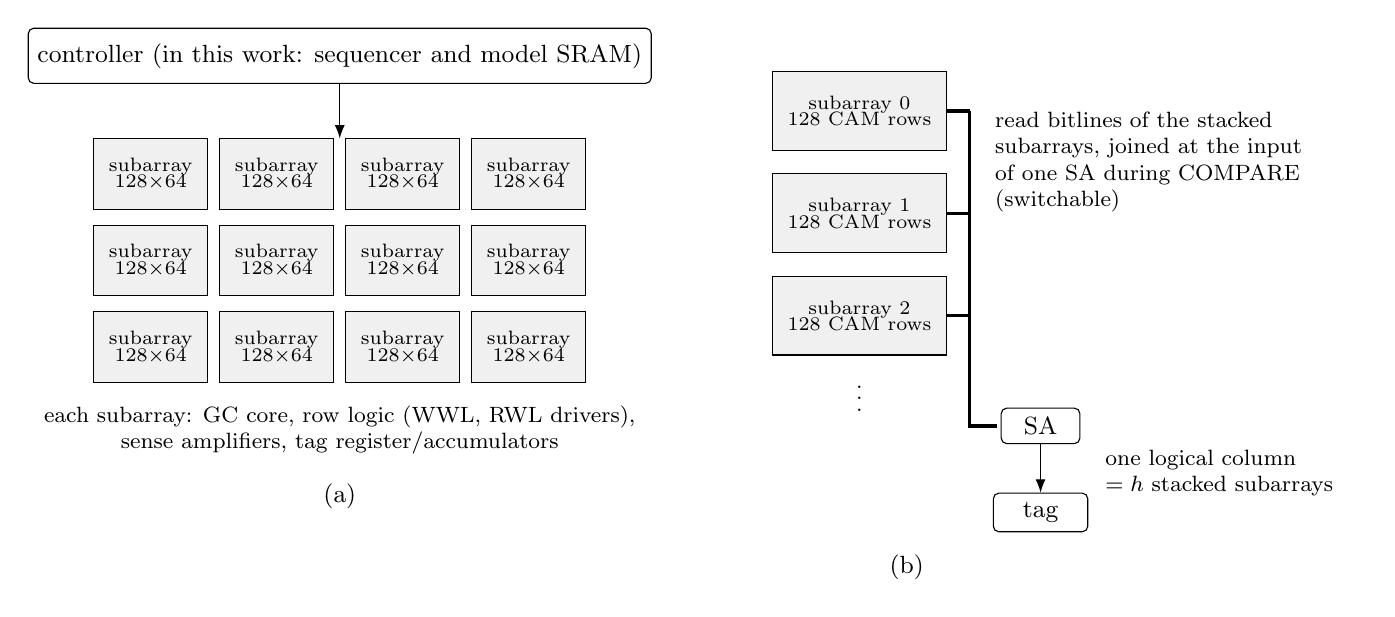
\begin{tikzpicture}[font=\small, >={Latex}]
\tikzset{sub/.style={draw, fill=black!6, minimum width=1.45cm, minimum height=0.9cm, font=\scriptsize, align=center},
         blk/.style={draw, rounded corners=2pt, align=center, fill=white}}
% (a) array of subarrays and controller
\node[blk, minimum width=6.6cm, minimum height=0.7cm] (ctl) at (2.4,4.1) {controller (in this work: sequencer and model SRAM)};
\foreach \i in {0,1,2,3} \foreach \j in {0,1,2} {
  \node[sub] (s\i\j) at (\i*1.6, 2.6-\j*1.1) {subarray\\[-2pt]$128{\times}64$};
}
\draw[->] (ctl.south) -- (2.4,3.05);
\node[font=\footnotesize, align=center] at (2.4,-0.65) {each subarray: GC core, row logic (WWL, RWL drivers),\\ sense amplifiers, tag register/accumulators};
\node at (2.4,-1.5) {(a)};
% (b) logical column built from stacked subarrays
\begin{scope}[xshift=9.0cm]
  \foreach \k/\y in {0/3.4, 1/2.1, 2/0.8} {
    \node[sub, minimum width=2.2cm, minimum height=1.0cm] (c\k) at (0,\y) {subarray $\k$\\[-2pt]128 CAM rows};
  }
  \foreach \y in {3.4, 2.1, 0.8} {\draw[very thick, black] (1.1,\y) -- (1.4,\y);}
  \node[font=\footnotesize] at (0,-0.15) {\vdots};
  \draw[very thick, black] (1.4,3.4) -- (1.4,-0.6) -- (1.75,-0.6);
  \node[blk, minimum width=1.0cm] (sa) at (2.3,-0.6) {SA};
  \node[blk, minimum width=1.2cm] (tag) at (2.3,-1.7) {tag};
  \draw[->] (sa) -- (tag);
  \node[anchor=west, align=left, font=\footnotesize, text width=4.6cm] at (1.6,2.75) {read bitlines of the stacked\\subarrays, joined at the input\\of one SA during COMPARE\\(switchable)};
  \node[anchor=west, align=left, font=\footnotesize] at (3.0,-1.2) {one logical column\\$= h$ stacked subarrays};
  \node at (0.6,-2.4) {(b)};
\end{scope}
\end{tikzpicture}}
\caption{(a) \gainp{} array organization, after~\cite{levi2026gainp}. (b) Logical column used in this work. During a compare, the read bitlines of $h$ vertically stacked subarrays are joined at the input of one sense amplifier. One compare thus spans all $h$ subarrays (one column shown). The local sense amplifiers of each subarray, used for refresh, are not shown.}
\label{fig:arch}
\end{figure}

The article also reports a power of 2.17~$\mu$W per bit at an operating frequency of 1~GHz, evaluated with a combination of silicon measurements and circuit simulation~\cite{levi2026gainp}. Table~\ref{tab:params7} uses this figure as 2.17~fJ per cell operation. This interpretation is ours.
The evaluation workbook of that study models the system at the same 1~GHz clock. This 1~ns cycle is shorter than the simulated 2~ns compare cycle.
The static power of 380~$\mu$W per Mbit is taken from the same workbook, which is not published. \hyp{We therefore treat it as an assumption.}

\section{Mapping FPTM onto \gainp{}}\label{sec:mapping}

We use the COMPARE and WRITE primitives of Section~\ref{sec:background} and a row READ.
COMPARE applies a pattern to a set of rows, masks all other rows and ORs the per-column match into the tag.
WRITE stores the tag into one row and clears the tag.
READ outputs one row.
\hyp{We assume that WRITE and READ, like COMPARE, take one cycle.}
We write $f \leftarrow \{q_1,\dots,q_k\}$ for $k$ compares with product terms $q_i$ followed by a write of $f$, which costs $k+1$ cycles.

\subsection{Exact clause simplification}\label{sec:norm}
Before code generation, each trained clause is simplified at compile time.
The rules below preserve Eq.~(\ref{eq:fptm}) exactly.
\begin{enumerate}
\item \emph{Conflicting literals.} If a clause includes both $x_i$ and $\lnot x_i$, exactly one of them fails for every input.
In FPTM, both literals are removed and $b_j$ decreases by one. If $b_j\le0$, the clause always scores zero and is removed.
In the strict TM, such a clause never fires and is removed.
FPTM training produces such clauses (Section~\ref{sec:results}).
\item \emph{Unreachable clamp.} If $b_j$ exceeds the number of remaining literals $n'_j$, the clamp in Eq.~(\ref{eq:fptm}) is never active. The excess $b_j-n'_j$ becomes a constant and $b_j\leftarrow n'_j$.
\item \emph{Constants.} Empty FPTM clauses score $\LF$. They and the constants of rule~2 are summed per class at compile time and written once as the initial value of the vote accumulators.
\item \emph{Unit budget.} If $b_j=1$, the score equals the strict conjunction of the remaining literals.
\end{enumerate}

\subsection{Mapping S: sample-stationary}\label{sec:mapS}
Each logical \gainp{} column holds one input sample in $F$ CAM rows, plus working rows.
The trained model is compiled into one data-independent program that the controller broadcasts to all columns.
\hyp{The program is not stored. A sequencer expands the sparse model, kept in an on-chip SRAM (M7), into the COMPARE and WRITE stream on the fly. Each literal and clause header is read once per batch, and the instruction pattern of a literal depends only on its position in the clause and on $b_j$.}
A batch is as wide as the number of available columns.
Inputs longer than the 128 CAM cells of a subarray occupy vertically adjacent subarrays.
We denote the number of stacked subarrays by $h=\lceil R/128\rceil$, where $R$ is the number of CAM rows of the program.
During COMPARE, the read bitlines of these subarrays are connected at the input of one sense amplifier, which feeds one tag register (Fig.~\ref{fig:arch}(b)).
The stacked subarrays thus form one logical column, and a single COMPARE spans all of them.
\hyp{Each subarray keeps its local sense amplifiers and tag registers, and the bitline join is switchable. Refresh opens the join and uses the local path, so all subarrays refresh in lockstep. The controller starts a refresh only after a WRITE, so that no partially accumulated tag is lost. In a WRITE, the tag drives the write bitlines of the subarray that holds the target row. The join switches are additional hardware. Their area and energy are not modelled.}
The same construction is used in Mapping~C.

\paragraph{Strict clauses}
A clause with $b_j=1$ is evaluated by a single COMPARE, followed by a WRITE to a temporary row $Q$ (2 cycles). The COMPARE pattern holds the required value of every included literal.
This uses the full associative search, independent of the clause length.

\paragraph{Fuzzy clauses, thermometer counter}
For $b_j\ge2$ we count misses with a saturating thermometer code $U_r=[m_j\ge r]$, $r=1,\dots,b_j$.
For the $t$-th literal, with input row $i$ and miss value $u$ (the complement of the required value), the update is
\begin{align}
U_r &\leftarrow \{U_r,\; U_{r-1}\wedge(x_i{=}u)\}, && r=\min(b_j,t),\dots,2,\\
U_1 &\leftarrow \{U_1,\; (x_i{=}u)\}.
\end{align}
Processing $r$ in descending order reads the old $U_{r-1}$.
Each level costs three cycles, so the literal costs $3\min(b_j,t)$ cycles.
Saturation is automatic. The score $s_j=b_j-\max\{r:U_r=1\}$, with the maximum taken as 0 if no $U_r$ is set, is then converted to binary. Bit $k$ of $s_j$ is the OR of the terms $U_m\wedge\lnot U_{m+1}$ over all $m=0,\dots,b_j$ with bit $k$ of $b_j-m$ set, where $U_0=1$ and $U_{b_j+1}=0$.

\paragraph{Fuzzy clauses, binary counter}
Alternatively, $m_j$ is accumulated in a binary counter.
The first counter bit fuses the literal test into the carry and sum terms.
After $t$ literals the counter needs $\lceil\log_2(t+1)\rceil$ bits, at 5 cycles per bit (3 for the top bit).
After the last literal, $b_j-m_j$ is computed with the constant $b_j$ folded into the product terms, and the borrow clamps negative results to zero.
The compiler emits both counters for each clause, counts their cycles and keeps the cheaper one.
The choice depends only on $n'_j$ and $b_j$, which are known after training.

\paragraph{Votes and decision}
Positive and negative scores are accumulated in two unsigned ripple-carry accumulators $P_c$ and $N_c$.
Their width grows with the running upper bound of the sum, so early additions are short.
After the last clause of a class, $V_c=P_c-N_c$ is formed by a ripple subtractor of at most 9 cycles per bit.
A running maximum $B$ and its class index $I$ are updated with a signed comparison and two conditional copies.
Strict ``greater than'' keeps the first maximum, as \texttt{argmax} does.
At the end, the $\lceil\log_2 K\rceil$ rows of $I$ are read out, where $K$ is the number of classes.
Algorithm~\ref{alg:mapS} summarizes the program.

\begin{algorithm}[t]
\caption{Sample-stationary FPTM program (broadcast to all columns).}
\label{alg:mapS}
\begin{algorithmic}[1]
\For{each class $c$}
  \State $P,N \gets$ compile-time constants of class $c$
  \For{each live clause $j$ of class $c$}
    \If{$b_j=1$} \State $Q\gets$ COMPARE(all literals of $j$); $Z\gets Q$
    \Else \State $Z\gets$ cheaper of thermometer and binary miss counter (Sec.~\ref{sec:mapS})
    \EndIf
    \State $P\gets P+Z$ if $j$ is positive, else $N\gets N+Z$
  \EndFor
  \State $V\gets P-N$; \textbf{if} $c=0$ \textbf{then} $B\gets V$, $I\gets0$ \textbf{else if} $V>B$ \textbf{then} $B\gets V$, $I\gets c$
\EndFor
\State read out $I$
\end{algorithmic}
\end{algorithm}

\subsection{Mapping C: clause-stationary}\label{sec:mapC}
Here each column holds one clause as a ternary pattern.
An included $x_i$ is stored as 1, an included $\lnot x_i$ as 0 and an excluded feature as ``don't care''.
The model is written once. The sample drives the searchlines, so no input data are written into the array.
Features that no clause uses are not stored, and their searchlines are not driven.

Conflicting literal pairs are removed and lower the stored budget (Section~\ref{sec:norm}).
If every live clause has $b_j=1$, one COMPARE over all used rows and one WRITE evaluate all clauses, for any number of clauses. One READ outputs the clause results.
For fuzzy clauses, the binary sense amplifier gives only match or mismatch per compare.
The miss count is therefore built feature by feature.
For each used feature, one COMPARE on that row and one WRITE produce the per-column match bit $\rho$.
A ``don't care'' cell always matches, so $\rho=0$ marks a miss.
The thermometer update of Section~\ref{sec:mapS} follows, with $\lnot\rho$ as the miss signal and at most $\LF$ levels.
After the last feature, the thermometer is converted to the binary miss count $m_j$.
Each column stores its own budget $b_j$ in $\lceil\log_2(\LF+1)\rceil$ rows, written with the model.
A borrow chain forms $s_j=\max(0,b_j-m_j)$, and the score rows are read out.

The class votes are sums over columns.
\gainp{} has no inter-column communication, so this reduction is not a native primitive.
\hyp{In Mapping~C, the reduction is performed outside the array. We report its operation count, one addition per live clause, but not its cost.}

\section{Evaluation Methodology}\label{sec:method}    
\subsection{Datasets}
We use three public datasets from different application domains (Table~\ref{tab:datasets}).
\begin{itemize}
\item \textbf{WOS-46985}~\cite{kowsari2017hdltex}: 46,985 Web of Science abstracts with 7 top-level domain labels (level~1).
We use a stratified 80/20 train/test split and hold out 10\% of the training split for validation.
Text is booleanized following the FPTM IMDb pipeline~\cite{hnilov2025code}, with n-grams up to length 2: a binary bag of unigrams and bigrams, then $\chi^2$ selection of 10,000 features.
The vocabulary and the $\chi^2$ selection are fitted on the training split, including its validation part, and never on the test split.
\item \textbf{ALeRCE}~\cite{sanchezsaez2021alerce}: the labeled set and light-curve features of the ALeRCE light curve classifier, with the 15 leaf classes of its taxonomy. The 152 features are thermometer-encoded at up to 7 quantile levels, plus missing-value bits, giving 1,172 Boolean inputs.
\item \textbf{NSL-KDD}~\cite{tavallaee2009nslkdd}: network connection records with 23 classes (normal traffic and 22 attack types). Numeric features are thermometer-encoded and categorical features one-hot encoded, giving 178 Boolean inputs. The test set is KDDTest+ restricted to attack types seen in training. It differs in distribution from the training set.
\end{itemize}
For ALeRCE and NSL-KDD, the train, validation and test splits and the booleanization come from the published TreeTM preparation code~\cite{treetm2026repo}, with seed 0. The TreeTM repository provides the preparation code but not the data, which are obtained from their original sources.
The WOS-46985 splits and the ALeRCE splits are stratified by class. The NSL-KDD training and validation splits are stratified by traffic category, and its test split is the fixed KDDTest+ set.

\begin{table}[!htbp]
\small
\centering
\caption{Datasets after booleanization.}
\label{tab:datasets}
\begin{tabular}{lllrrrr}
\toprule
Dataset & Domain & Classes & Bits & Train & Val. & Test \\
\midrule
WOS-46985 & Scientific text & 7 & 10,000 & 33,829 & 3,759 & 9,397 \\
ALeRCE & Astronomy & 15 & 1,172 & 88,916 & 9,880 & 24,700 \\
NSL-KDD & Network security & 23 & 178 & 113,375 & 12,598 & 18,794 \\
\bottomrule
\end{tabular}
\end{table}

\subsection{Models and training}
We ported \texttt{FuzzyPatternTM.jl} line by line to Python with Numba.
Clause evaluation, vote, both feedback types, include thresholds and state bounds follow the Julia code.
The port therefore contains the three FPTM modifications and the two trainer details of Section~\ref{sec:background}.


We compare three model families.
\begin{itemize}
\item \textbf{FPTM}, with 2, 10, 20, 40 and 100 clauses per class.
$\LF$ and $L$ decrease as the clause count grows (Table~\ref{tab:hyper}).
\item \textbf{FPTM with $\LF=1$}, i.e.\ the FPTM trainer with strict clause voting. We refer to them as strict models.
We use 200, 400, 600 and 1,000 clauses per class on ALeRCE and NSL-KDD, and 200 and 400 on WOS-46985.
\item \textbf{Vanilla TM}, Granmo's multiclass TM in the \texttt{pyTsetlinMachine} package~\cite{pytsetlin}, with 200 and 1,000 clauses per class on ALeRCE and NSL-KDD and 400 on WOS-46985.

\end{itemize}
The $\LF=1$ family shares the FPTM trainer and differs from FPTM in the clause vote.
It still differs from FPTM in clause count, $T$, $L$ and include limit. It is therefore not a controlled ablation of the fuzzy vote.
Differences between the $\LF=1$ family and the vanilla TM combine the trainer differences of Section~\ref{sec:background} with different hyperparameters. We do not attribute them to a single cause.

Table~\ref{tab:hyper} lists all hyperparameters.
They follow the examples of the FPTM reference code and common TM settings. No hyperparameter search was performed for the main experiments. The final settings were fixed after an earlier single-seed round, whose validation and test results were known at that time. \wosnew{Section~S1 of the supplementary material describes this round and its baselines.}

Every run trains for at most 50 epochs and stops after 10 epochs without a new best validation accuracy.
The epoch with the best validation accuracy is kept, and its test accuracy is measured once.
Each configuration is trained with three seeds.
Because of training time, the 1,000-clause models on ALeRCE and NSL-KDD and the vanilla TM on WOS-46985 use one seed.
We report the mean and the sample standard deviation over seeds.
The test accuracy is that of the exported clause set, i.e.\ the model that \gainp{} executes.
\wosnew{Section~S2 of the supplementary material gives further training details.}

\wosnew{\textit{Energy-oriented hyperparameters.} The hyperparameters of Table~\ref{tab:hyper} aim at accuracy. We call them accuracy-oriented.
After the main experiments, one of the authors chose new values for the FPTM and strict models of each dataset with the reference FPTM implementation~\cite{hnilov2025code}. The tuning used the validation split only. We trained the reported models with our port.
Its goal was a low density of included literals at an acceptable, not maximum, accuracy. We call these settings energy-oriented.
On ALeRCE, the threshold is $T=\sqrt{C\,\LF/2}$~\cite{hnilov2025fptm}, rounded to an integer, with $C$ clauses per class.
There, $L$, $\LF$ and $S$ were chosen for 2, 20 and 200 clauses per class and interpolated or extrapolated for the other sizes.
On NSL-KDD and WOS-46985, the values were chosen per model. Table~\ref{tab:energyhp} lists all values.
Each energy-oriented model trains for at least 300 epochs, and the epoch is again selected on the validation split.
ALeRCE and WOS-46985 use two runs per model. Both use the same sample order and differ in the random sequence of the feedback steps. The first stops at 300 epochs. The second continues while the validation accuracy improves and stops after 50 epochs without a new best. No model of the second runs improved after epoch 300.
NSL-KDD uses one 300-epoch run. The include limit is 200, except for the strict ALeRCE and WOS-46985 models, which use 128.
Taking the epoch-300 model instead of the best validation epoch changes the test accuracy by at most 0.5 points on ALeRCE and NSL-KDD.}

\begin{table}[!htbp]
\footnotesize
\setlength{\tabcolsep}{4pt}
\centering
\caption{\wosnew{Accuracy-oriented hyperparameters and number of seeds. W, A, N: WOS-46985, ALeRCE, NSL-KDD. $S$: FPTM specificity divisor, which sets $d=\mathrm{round}(F/S)$, with $S=1{,}000$, 200 and 100 on W, A and N. $s$: vanilla TM specificity. Strict: FPTM trainer with $\LF=1$. Table~S1 of the supplementary material lists the best epoch of each run.}}
\label{tab:hyper}
\begin{tabular}{lrrrrrrr}
\toprule
Model & Cl./class & $\LF$ & $L$ & $T$ & $S$ or $s$ & Incl.\ limit & Datasets (seeds) \\
\midrule
FPTM & 2 & 32 & 64 & 10 & $S$ & 200 & W, A, N (3) \\
FPTM & 10 & 16 & 64 & 20 & $S$ & 200 & W, A, N (3) \\
FPTM & 20 & 8 & 32 & 20 & $S$ & 200 & W, A, N (3) \\
FPTM & 40 & 8 & 16 & 32 & $S$ & 200 & W, A, N (3) \\
FPTM & 100 & 4 & 16 & 50 & $S$ & 200 & W, A, N (3) \\
Strict & 200 & 1 & 16 & 50 & $S$ & 128 & W, A, N (3) \\
Strict & 400 & 1 & 16 & 75 & $S$ & 128 & W, A, N (3) \\
Strict & 600 & 1 & 16 & 90 & $S$ & 128 & A, N (3) \\
Strict & 1,000 & 1 & 16 & 100 & $S$ & 128 & A, N (1) \\
Vanilla TM & 200 & n/a & n/a & 50 & $s=10$ & n/a & A, N (3) \\
Vanilla TM & 400 & n/a & n/a & 100 & $s=10$ & n/a & W (1) \\
Vanilla TM & 1,000 & n/a & n/a & 100 & $s=10$ & n/a & A, N (1) \\
\bottomrule
\end{tabular}
\end{table}

\subsection{\gainp{} evaluation}\label{sec:eval}
For each trained model, the compilers of Section~\ref{sec:mapping} generate the \gainp{} programs of both mappings.
A functional simulator executes them with the COMPARE, WRITE and READ semantics of Section~\ref{sec:mapping}, including ternary storage for Mapping~C.
For every run, the in-array prediction was compared with an independent NumPy reference of the trained model. Mapping~S was checked on the first 1,500 test samples and Mapping~C on the first 200 test samples of each dataset.

The cycle and row counts of each program do not depend on the data.

\begin{table}[!htbp]
\small
\centering
\caption{\gainp{} parameters: 16~nm reference values based on~\cite{levi2026gainp} (Section~\ref{sec:gainp}) and 7~nm corners.}
\label{tab:params7}
\begin{tabular}{lrrrr}
\toprule
 & 16~nm & 16~nm & 7~nm & 7~nm \\
Parameter & circuit & system & conservative & optimistic \\
\midrule
Compare cycle (ns) & 2.00 & 1.00 & \hyp{1.48} & \hyp{1.00} \\
Energy per cell operation (fJ) & 10.40 & \hyp{2.17} & \hyp{7.70} & \hyp{0.76} \\
Subarray macro area ($\mu$m$^2$) & 1890 & 1890 & \hyp{729} & \hyp{729} \\
Gain-cell area ($\mu$m$^2$) & 0.0820 & 0.0820 & \hyp{0.0316} & \hyp{0.0316} \\
Static power ($\mu$W/Mbit) & \hyp{380} & \hyp{380} & \hyp{380} & \hyp{133} \\
Refresh period ($\mu$s) & \hyp{52.96} & \hyp{52.96} & \hyp{52.96} & \hyp{52.96} \\
\bottomrule
\end{tabular}
\end{table}

Latency, energy and area follow from the executed programs and the parameters of Table~\ref{tab:params7}. The 7~nm design is evaluated at a conservative and an optimistic corner, given by the two 7~nm columns of Table~\ref{tab:params7}.
The primary evaluation uses the two 7~nm corners. The 16~nm values serve as a reference.
\begin{itemize}
\item Latency: cycles $\times$ cycle time, plus refresh stalls.
\item Dynamic energy: the sum over cycles of the number of unmasked rows, times the number of active columns, times the energy per cell operation.
\item Static energy: the static power per Mbit of gain cells occupied by the sample (Mapping~S) or by the model (Mapping~C), times the latency.
\item Controller energy: sequencer cycles and model-store reads (M6).
\item Area: number of occupied subarrays $\times$ the subarray macro area, plus the model SRAM in Mapping~S (M7). In Mapping~S, a stack of $h$ subarrays forms 64 logical columns and holds 64 samples.
\end{itemize}
\hyp{The following assumptions are ours and are not taken from~\cite{levi2026gainp}.
(M1) WRITE and READ take one cycle and cost the same energy per cell as COMPARE.
(M2) Dynamic energy scales with the number of unmasked rows, and masked rows cost nothing. Section~\ref{sec:sens} reports the alternative that charges one cell operation per column and cycle.
(M3) Refresh is applied every 52.96~$\mu$s (Table~\ref{tab:params7}). One refresh reads and rewrites all gain-cell rows of every occupied subarray in lockstep, through the local sense amplifiers. It stalls the array for 512 cycles and costs two cell operations per CAM cell.} \wosnew{Section~S3 of the supplementary material gives the details and discusses the tail of the retention time distribution.} \hyp{
(M4) In Mapping~S, loading a batch writes one input row per cycle, $F$ cycles in total. Off-chip input bandwidth is not modelled. Load time is included in the throughput. The load energy, i.e., the cell, sequencer and static energy of the load cycles, is excluded from the reported energy. It is at most 0.39~nJ (conservative) per sample, on WOS-46985, and at most 11\% of the reported energy.} \hyp{
(M5) In Mapping~C, the vote reduction outside the array is excluded from latency and energy.
(M6) A sequencer generates the COMPARE, WRITE and READ stream (Section~\ref{sec:mapS}). Its energy is charged per issued cycle, including refresh cycles, and per 32-bit read of the model store. Each read returns two 16-bit entries.} A 32-bit SRAM access costs 5~pJ in 45~nm CMOS~\cite{han2016deep}. \hyp{Both costs are anchored at this value, independent of the store size. The 16~nm reference points use 5~pJ. At the 7~nm corners, we assume 3.70~pJ (conservative) and 1.75~pJ (optimistic). The 45~nm to 16~nm reduction is not applied, so these values are upper estimates. In Mapping~S, one sequencer and one model store serve a macro of 256 subarrays, which holds $\lfloor 256/h\rfloor$ stacks of 64 samples each. The per-batch controller energy is shared by all samples of the macro. We assume a prefetch buffer large enough that the store does not stall the array. Its area and energy are not modelled.} \wosnew{Section~S3 of the supplementary material gives its sizing.} \hyp{ In Mapping~C, the controller energy is charged to each sample. Its sequencer keeps only the list of used features, whose area is not modelled.
(M7) The model store holds one 16-bit entry per included literal and one per clause. It is a high-density SRAM with the 7~nm cell area of~\cite{wu2016n7} and the 75\% array efficiency of the \gainp{} macro. Its area is added to the Mapping~S area. The sequencer logic area is not modelled. The leakage of the model SRAM is not modelled either.} \wosnew{Section~S3 of the supplementary material estimates this leakage. It would add at most} \hyp{24\%} \wosnew{(conservative) and} \hyp{27\%} \wosnew{(optimistic) to the Mapping~S energy, and} \hyp{0.4\% to 0.6\%} \wosnew{for the 20-clause ALeRCE FPTM.}
\section{Results}\label{sec:results}

\subsection{Functional verification}
For all 80 training runs, the executed Mapping~S program reproduced the reference prediction on each of the first 1,500 test samples.
The executed Mapping~C program, followed by the vote reduction in NumPy, reproduced it on each of the first 200 test samples.
The compile-time simplification of Section~\ref{sec:norm} is exact by construction, and these checks confirm it on every model.
Conflicting literals do occur in FPTM. For example, 32 of the 46 clauses of the seed-0 2-clause NSL-KDD model include some feature both plainly and negated.

\subsection{Accuracy and model size}\label{sec:accuracy}
Table~\ref{tab:accuracy} lists validation and test accuracy, the number of included literals and the model size.
The model size assumes a sparse encoding with one feature index and one polarity bit per included literal.
Values are the mean and standard deviation over seeds.

\begin{table}[!htbp]
\small
\centering
\caption{Accuracy and model size, mean $\pm$ standard deviation over seeds (Table~\ref{tab:hyper}). Test accuracy is that of the exported clause set at the epoch with the best validation accuracy. Literals: included literals over all clauses. Strict: FPTM trainer with $\LF=1$.}
\label{tab:accuracy}
\begin{tabular}{lrrrrr}
\toprule
Model & Cl./class & Val.\ acc.\ (\%) & Test acc.\ (\%) & Literals & Size (KiB) \\
\midrule
\multicolumn{6}{l}{\textit{WOS-46985}} \\
FPTM & 2 & 81.64 $\pm$ 0.55 & 81.98 $\pm$ 0.45 & 16,466 & 30.2 \\
FPTM & 10 & 86.46 $\pm$ 0.25 & 85.96 $\pm$ 0.06 & 56,163 & 102.8 \\
FPTM & 20 & 87.91 $\pm$ 0.23 & 87.82 $\pm$ 0.33 & 59,753 & 109.4 \\
FPTM & 40 & 88.44 $\pm$ 0.20 & 88.09 $\pm$ 0.04 & 92,907 & 170.1 \\
FPTM & 100 & 89.62 $\pm$ 0.15 & 89.50 $\pm$ 0.01 & 150,218 & 275.1 \\
Strict & 200 & 90.49 $\pm$ 0.06 & 90.87 $\pm$ 0.09 & 103,091 & 188.8 \\
Strict & 400 & 90.53 $\pm$ 0.14 & 90.87 $\pm$ 0.09 & 183,056 & 335.2 \\
Vanilla TM & 400 & 78.27 & 78.26 & 2,984,562 & 5,464.9 \\
\midrule
\multicolumn{6}{l}{\textit{ALeRCE}} \\
FPTM & 2 & 90.55 $\pm$ 0.35 & 90.54 $\pm$ 0.29 & 2,561 & 3.8 \\
FPTM & 10 & 92.90 $\pm$ 0.11 & 92.84 $\pm$ 0.14 & 10,537 & 15.4 \\
FPTM & 20 & 93.26 $\pm$ 0.05 & 93.23 $\pm$ 0.10 & 11,776 & 17.2 \\
FPTM & 40 & 93.76 $\pm$ 0.07 & 93.65 $\pm$ 0.04 & 19,011 & 27.8 \\
FPTM & 100 & 93.77 $\pm$ 0.06 & 93.59 $\pm$ 0.06 & 33,623 & 49.3 \\
Strict & 200 & 90.81 $\pm$ 0.08 & 90.92 $\pm$ 0.14 & 50,933 & 74.6 \\
Strict & 400 & 91.80 $\pm$ 0.07 & 92.12 $\pm$ 0.14 & 105,409 & 154.4 \\
Strict & 600 & 92.42 $\pm$ 0.08 & 92.63 $\pm$ 0.08 & 160,015 & 234.4 \\
Strict & 1,000 & 93.13 & 93.28 & 273,580 & 400.8 \\
Vanilla TM & 200 & 78.80 $\pm$ 0.42 & 78.65 $\pm$ 0.55 & 314,385 & 460.5 \\
Vanilla TM & 1,000 & 91.53 & 91.43 & 912,839 & 1,337.2 \\
\midrule
\multicolumn{6}{l}{\textit{NSL-KDD}} \\
FPTM & 2 & 96.19 $\pm$ 0.56 & 84.11 $\pm$ 0.26 & 3,838 & 4.2 \\
FPTM & 10 & 98.23 $\pm$ 0.04 & 85.63 $\pm$ 0.14 & 15,595 & 17.1 \\
FPTM & 20 & 98.62 $\pm$ 0.06 & 85.94 $\pm$ 0.22 & 18,117 & 19.9 \\
FPTM & 40 & 98.74 $\pm$ 0.04 & 86.40 $\pm$ 0.02 & 34,685 & 38.1 \\
FPTM & 100 & 98.79 $\pm$ 0.00 & 86.26 $\pm$ 0.01 & 69,400 & 76.2 \\
Strict & 200 & 98.54 $\pm$ 0.04 & 85.82 $\pm$ 0.07 & 91,111 & 100.1 \\
Strict & 400 & 98.71 $\pm$ 0.07 & 86.12 $\pm$ 0.18 & 216,928 & 238.3 \\
Strict & 600 & 98.79 $\pm$ 0.03 & 86.23 $\pm$ 0.06 & 348,593 & 383.0 \\
Strict & 1,000 & 98.91 & 86.02 & 436,996 & 480.1 \\
Vanilla TM & 200 & 93.23 $\pm$ 0.83 & 81.22 $\pm$ 2.18 & 407,988 & 448.2 \\
Vanilla TM & 1,000 & 98.21 & 86.08 & 1,385,591 & 1,522.3 \\
\bottomrule
\end{tabular}
\end{table}

On ALeRCE, FPTM reaches 90.54\% $\pm$ 0.29\% with 2 clauses per class and 93.23\% $\pm$ 0.10\% with 20 clauses per class.
The strict $\LF=1$ models need 1,000 clauses per class for 93.28\%. With 600 clauses per class they reach 92.63\% $\pm$ 0.08\%.
The 20-clause FPTM uses 11,776 literals on average, $13.6\times$ fewer than the 600-clause $\LF=1$ model (160,015).
The vanilla TM reaches 78.65\% $\pm$ 0.55\% with 200 and 91.43\% with 1,000 clauses per class.

On NSL-KDD, all models trained with the FPTM trainer and at least 10 clauses per class lie between 85.63\% and 86.40\% test accuracy.
The validation accuracy of the same models lies between 98.23\% and 98.91\%. Validation and test rankings do not agree, because KDDTest+ differs in distribution from the training data.
Test differences below about 0.5 points on NSL-KDD should therefore not be read as a ranking.
The vanilla TM reaches 81.22\% $\pm$ 2.18\% with 200 and 86.08\% with 1,000 clauses per class.

On WOS-46985, the strict $\LF=1$ models reach the highest accuracy, 90.87\% $\pm$ 0.09\% with both 200 and 400 clauses per class.
FPTM improves with the clause count, from 81.98\% $\pm$ 0.45\% with 2 clauses to 89.50\% $\pm$ 0.01\% with 100 clauses per class.
FPTM clauses on WOS are long. With the hyperparameters of Table~\ref{tab:hyper}, the 2-clause models carry about 1,050 to 1,300 literals per clause, mostly negated word literals.
The vanilla TM with 400 clauses per class reaches 78.26\% (one seed).
No hyperparameter search was performed for the vanilla TM on any dataset. Its results should not be read as the capability of the vanilla TM.

\subsection{7~nm \gainp{} cost, Mapping~S}
Table~\ref{tab:mapS} gives the program length, the batch latency, the energy per sample and the throughput per unit area for Mapping~S at the two 7~nm corners.
\wosnew{Fig.~S1 of the supplementary material plots test accuracy against energy per sample at the optimistic corner for all three datasets.}
The cycle count is a property of the program and does not depend on the process. It varies between seeds because the trained clauses differ.

\begin{sidewaystable}
\footnotesize
\setlength{\tabcolsep}{4pt}
\centering
\caption{Mapping~S (sample-stationary) at the 7~nm corners, mean $\pm$ standard deviation over seeds where shown. Rows/col.: CAM rows per logical column. Subarrays: stacked subarrays per logical column. Latency includes refresh. Energy includes dynamic, refresh, gain-cell static and controller energy (M6). It excludes input loading (M4) and model-SRAM leakage (M7). Throughput includes input loading and is given per mm$^2$ of occupied subarrays and model SRAM (M7) of a 256-subarray macro.}
\label{tab:mapS}
\begin{tabular}{lrrrrrrrr}
\toprule
\multirow{2}{*}{Model (cl./class)} & Rows & Sub- & Cycles & \multicolumn{2}{c}{Batch latency ($\mu$s)} & \multicolumn{2}{c}{Energy (nJ/sample)} & Thr., opt. \\
 & /col. & arrays & ($\times10^3$) & cons. & opt. & cons. & opt. & (M/s/mm$^2$) \\
\midrule
\multicolumn{9}{l}{\textit{WOS-46985}} \\
FPTM (2) & 10,060 & 79 & 729.6 $\pm$ 86.5 & \hyp{1,096} & \hyp{737} & \hyp{35.06 $\pm$ 4.15} & \hyp{9.871 $\pm$ 1.168} & \hyp{1.43} \\
FPTM (10) & 10,083 & 79 & 2,370.7 $\pm$ 200.0 & \hyp{3,562} & \hyp{2,394} & \hyp{112.41 $\pm$ 9.72} & \hyp{31.936 $\pm$ 2.715} & \hyp{0.392} \\
FPTM (20) & 10,064 & 79 & 1,404.3 $\pm$ 73.0 & \hyp{2,110} & \hyp{1,418} & \hyp{64.42 $\pm$ 3.34} & \hyp{18.800 $\pm$ 0.976} & \hyp{0.650} \\
FPTM (40) & 10,068 & 79 & 2,196.5 $\pm$ 383.9 & \hyp{3,301} & \hyp{2,218} & \hyp{100.81 $\pm$ 17.58} & \hyp{29.409 $\pm$ 5.135} & \hyp{0.390} \\
FPTM (100) & 10,048 & 79 & 1,821.2 $\pm$ 202.8 & \hyp{2,737} & \hyp{1,839} & \hyp{83.73 $\pm$ 9.31} & \hyp{24.665 $\pm$ 2.747} & \hyp{0.405} \\
Strict (200) & 10,037 & 79 & 41.5 $\pm$ 0.0 & \hyp{62.4} & \hyp{41.9} & \hyp{3.77 $\pm$ 0.02} & \hyp{1.110 $\pm$ 0.006} & \hyp{15.9} \\
Strict (400) & 10,041 & 79 & 95.7 $\pm$ 0.0 & \hyp{144} & \hyp{96.7} & \hyp{7.74 $\pm$ 0.31} & \hyp{2.267 $\pm$ 0.094} & \hyp{6.44} \\
Vanilla TM (400) & 10,041 & 79 & 95.7 & \hyp{144} & \hyp{96.6} & \hyp{56.34} & \hyp{17.161} & \hyp{0.951} \\
\midrule
\multicolumn{9}{l}{\textit{ALeRCE}} \\
FPTM (2) & 1,231 & 10 & 70.3 $\pm$ 4.0 & \hyp{106} & \hyp{71.0} & \hyp{1.19 $\pm$ 0.07} & \hyp{0.192 $\pm$ 0.011} & \hyp{121} \\
FPTM (10) & 1,233 & 10 & 276.1 $\pm$ 8.6 & \hyp{415} & \hyp{279} & \hyp{4.65 $\pm$ 0.14} & \hyp{0.754 $\pm$ 0.024} & \hyp{30.4} \\
FPTM (20) & 1,237 & 10 & 270.1 $\pm$ 10.0 & \hyp{406} & \hyp{273} & \hyp{4.42 $\pm$ 0.14} & \hyp{0.726 $\pm$ 0.025} & \hyp{30.9} \\
FPTM (40) & 1,241 & 10 & 423.2 $\pm$ 37.9 & \hyp{636} & \hyp{427} & \hyp{6.84 $\pm$ 0.55} & \hyp{1.129 $\pm$ 0.095} & \hyp{19.4} \\
FPTM (100) & 1,221 & 10 & 457.1 $\pm$ 22.0 & \hyp{687} & \hyp{462} & \hyp{6.73 $\pm$ 0.31} & \hyp{1.161 $\pm$ 0.055} & \hyp{17.1} \\
Strict (200) & 1,210 & 10 & 89.0 $\pm$ 0.0 & \hyp{134} & \hyp{89.9} & \hyp{1.90 $\pm$ 0.00} & \hyp{0.304 $\pm$ 0.000} & \hyp{82.4} \\
Strict (400) & 1,214 & 10 & 205.3 $\pm$ 0.0 & \hyp{308} & \hyp{207} & \hyp{4.28 $\pm$ 0.01} & \hyp{0.686 $\pm$ 0.001} & \hyp{31.2} \\
Strict (600) & 1,218 & 10 & 332.3 $\pm$ 0.0 & \hyp{499} & \hyp{335} & \hyp{6.84 $\pm$ 0.02} & \hyp{1.098 $\pm$ 0.003} & \hyp{17.0} \\
Strict (1,000) & 1,218 & 10 & 602.3 & \hyp{905} & \hyp{608} & \hyp{12.27} & \hyp{1.969} & \hyp{7.54} \\
Vanilla TM (200) & 1,210 & 10 & 88.9 $\pm$ 0.0 & \hyp{134} & \hyp{89.7} & \hyp{4.23 $\pm$ 0.45} & \hyp{0.648 $\pm$ 0.066} & \hyp{48.4} \\
Vanilla TM (1,000) & 1,218 & 10 & 600.7 & \hyp{903} & \hyp{606} & \hyp{17.90} & \hyp{2.800} & \hyp{3.67} \\
\midrule
\multicolumn{9}{l}{\textit{NSL-KDD}} \\
FPTM (2) & 237 & 2 & 96.5 $\pm$ 0.4 & \hyp{145} & \hyp{97.5} & \hyp{1.29 $\pm$ 0.00} & \hyp{0.147 $\pm$ 0.001} & \hyp{445} \\
FPTM (10) & 243 & 2 & 387.3 $\pm$ 6.6 & \hyp{582} & \hyp{391} & \hyp{5.15 $\pm$ 0.09} & \hyp{0.589 $\pm$ 0.010} & \hyp{107} \\
FPTM (20) & 244 & 2 & 403.3 $\pm$ 24.9 & \hyp{606} & \hyp{407} & \hyp{5.05 $\pm$ 0.26} & \hyp{0.583 $\pm$ 0.031} & \hyp{102} \\
FPTM (40) & 248 & 2 & 741.4 $\pm$ 140.4 & \hyp{1,114} & \hyp{749} & \hyp{8.96 $\pm$ 1.47} & \hyp{1.039 $\pm$ 0.174} & \hyp{54.5} \\
FPTM (100) & 228 & 2 & 911.6 $\pm$ 57.5 & \hyp{1,370} & \hyp{920} & \hyp{10.03 $\pm$ 0.60} & \hyp{1.184 $\pm$ 0.072} & \hyp{39.2} \\
Strict (200) & 217 & 2 & 136.6 $\pm$ 0.0 & \hyp{205} & \hyp{138} & \hyp{2.46 $\pm$ 0.07} & \hyp{0.279 $\pm$ 0.008} & \hyp{246} \\
Strict (400) & 221 & 2 & 314.7 $\pm$ 0.1 & \hyp{473} & \hyp{318} & \hyp{5.74 $\pm$ 0.47} & \hyp{0.650 $\pm$ 0.051} & \hyp{81.9} \\
Strict (600) & 225 & 2 & 509.5 $\pm$ 0.0 & \hyp{766} & \hyp{514} & \hyp{9.28 $\pm$ 0.64} & \hyp{1.051 $\pm$ 0.070} & \hyp{40.6} \\
Strict (1,000) & 225 & 2 & 923.0 & \hyp{1,387} & \hyp{932} & \hyp{15.29} & \hyp{1.738} & \hyp{19.5} \\
Vanilla TM (200) & 217 & 2 & 136.5 $\pm$ 0.1 & \hyp{205} & \hyp{138} & \hyp{4.97 $\pm$ 0.07} & \hyp{0.553 $\pm$ 0.007} & \hyp{140} \\
Vanilla TM (1,000) & 225 & 2 & 922.0 & \hyp{1,386} & \hyp{931} & \hyp{22.80} & \hyp{2.558} & \hyp{8.82} \\
\bottomrule
\end{tabular}
\end{sidewaystable}


A strict clause costs one COMPARE whatever its length.
A fuzzy clause costs a miss count that grows with its length.
The trade-off is therefore decided by how many strict clauses an FPTM clause replaces.

On ALeRCE, above about 92.5\% accuracy, FPTM is more accurate and needs fewer cycles and less energy.
The 20-clause FPTM (93.23\%) needs 270.1k cycles and \hyp{4.42~nJ (conservative) or 0.73~nJ (optimistic)} per sample, including the controller.
The 600-clause $\LF=1$ model (92.63\%) needs 332.3k cycles and \hyp{6.84~nJ or 1.10~nJ}.
The 40-clause FPTM (93.65\%) needs 423.2k cycles and \hyp{6.84~nJ or 1.13~nJ}. The 1,000-clause $\LF=1$ model (93.28\%) needs 602.3k cycles and \hyp{12.27~nJ or 1.97~nJ}.
At the low end, the 200-clause $\LF=1$ model is 0.38 points more accurate on average than the 2-clause FPTM, about 1.3 standard deviations of the FPTM runs. It needs $1.27\times$ more cycles and \hyp{$1.6\times$} more energy.

On NSL-KDD, at moderate accuracy, the strict models need fewer cycles and less energy.
The 200-clause $\LF=1$ model (85.82\%) needs 136.6k cycles and \hyp{2.46~nJ or 0.28~nJ}, against 403.3k cycles and \hyp{5.05~nJ or 0.58~nJ} for the 20-clause FPTM (85.94\%).
At the top of the accuracy range, the 40-clause FPTM (86.40\%) and the 600-clause $\LF=1$ model (86.23\%) need similar energy. At the conservative corner, they need \hyp{8.96~nJ and 9.28~nJ}, although the FPTM needs more cycles.

On WOS-46985, the strict model is more accurate and needs fewer cycles and less energy.
The 200-clause $\LF=1$ model needs 41.5k cycles and \hyp{3.77~nJ or 1.11~nJ} for 90.87\%.
The 100-clause FPTM needs 1,821k cycles and \hyp{83.7~nJ or 24.7~nJ} for 89.50\%.
Long FPTM clauses make the miss counts expensive. The 10,000-bit inputs also need 79 stacked subarrays per logical column, which raises the static energy and lowers the throughput density. \hyp{Only three such stacks fit in a 256-subarray macro, so the controller energy is shared by fewer samples.}

\subsection{7~nm \gainp{} cost, Mapping~C}\label{sec:mapCres}
\wosnew{Table~S2 of the supplementary material reports Mapping~C in full.}
Here a strict model evaluates all its clauses in one COMPARE, one WRITE and one READ, i.e., 3 cycles.
Its area, however, grows with the clause count. The 1,000-clause $\LF=1$ ALeRCE model needs 15,000 clause columns and \hyp{1.71~mm$^2$}.
Its 15,000 clause outputs must also be reduced outside the array.
The 20-clause FPTM fits in \hyp{0.036~mm$^2$} and leaves 300 values to reduce, but needs 30,258 cycles per sample because the miss count is built feature by feature.
\wosnew{The 20-clause FPTM needs} \hyp{222~nJ or 65.9~nJ} \wosnew{per sample, against} \hyp{136~nJ or 13.4~nJ} \wosnew{for the 1,000-clause strict model.}
Per sample, Mapping~C needs more energy than Mapping~S for every FPTM and strict model. Each sample activates the whole model array, and the controller energy is not shared between samples.


\subsection{Comparison with CPU inference and TM hardware}\label{sec:compare}
To our knowledge, no hardware implementation of FPTM has been reported. The FPTM paper reports CPU inference only~\cite{hnilov2025fptm}.
We therefore compare \gainp{} with FPTM and TM inference on a CPU, and with published hardware accelerators for the vanilla TM and other TM variants.

\paragraph{CPU}
We ran every exported model on one core of an Intel Xeon processor at 2.10~GHz.
\wosnew{We bound the CPU energy from below by assuming that the active core draws at least 1~W.}
\hyp{For this comparison, the \gainp{} energy includes input loading (M4), because the CPU time includes input packing. Under this bound, the fastest single-thread CPU kernel needs between $63\times$ and about $7{,}100\times$ more energy per classification than \gainp{} at the conservative corner, for every model. For the 20-clause ALeRCE FPTM, the ratio is about $810\times$.}
\wosnew{Section~S6 of the supplementary material gives the CPU times, the kernels and the timing protocol.}

\paragraph{TM hardware accelerators}
Table~\ref{tab:tmhw} lists published TM accelerators that report energy or throughput, together with representative \gainp{} results.
The comparison is not like for like. The designs differ in dataset, TM variant, model size and technology node, and several of them report simulated rather than measured results.
Our \gainp{} values are design results for a commercial 7~nm process. This design has not been fabricated. Their energy includes the controller and excludes feature extraction, off-chip input transfer and input loading into the array. Their throughput includes input loading.
\hyp{Over all 30 configurations in Mapping~S and both corners, the \gainp{} energy per classification is 0.15 to 112~nJ, excluding model-SRAM leakage (M7).} The reported TM ASICs and in-memory designs span 30.6~pJ to 191~nJ, and the reported FPGA accelerators 0.6 to 73.6~$\mu$J. \hyp{The \gainp{} energy thus lies within the first range. It is at least $5.3\times$ below the FPGA accelerators, and at least $33\times$ below them for the four listed models.
The occupied subarrays of one 256-subarray macro and its model SRAM take 0.19 to 0.72~mm$^2$, without the sequencer logic. The macro would classify $1.8\times10^6$ to $4.0\times10^7$ samples per second for the listed models.} The 65~nm ASIC of~\cite{tunheim2026asic} classifies $6.03\times10^4$ samples per second in 2.7~mm$^2$.

\begin{sidewaystable}
\footnotesize
\setlength{\tabcolsep}{4pt}
\centering
\caption{Published TM inference hardware and the 7~nm \gainp{} design (not fabricated). Energy and throughput as reported by each design. n/r: not reported. Model: TM variant, with clauses per class in parentheses. For \gainp{}, energy includes the controller, excludes input loading and model-SRAM leakage, and is given at the conservative and optimistic corners. Throughput is given at the conservative corner for one 256-subarray macro, with its area including the model SRAM.}
\label{tab:tmhw}
\scriptsize
\setlength{\tabcolsep}{3pt}
\begin{tabular}{>{\raggedright\arraybackslash}p{3.0cm}>{\raggedright\arraybackslash}p{3.2cm}>{\raggedright\arraybackslash}p{2.7cm}>{\raggedright\arraybackslash}p{2.4cm}r>{\raggedright\arraybackslash}p{2.4cm}>{\raggedright\arraybackslash}p{2.9cm}}
\toprule
Design & Platform & Model & Dataset & Acc.\ (\%) & Energy/classif. & Classif./s \\
\midrule
Wheeldon et al.~\cite{wheeldon2020learning} & ASIC, 65~nm, layout & Vanilla TM (20) & Iris & n/r$^{a}$ & 30.6~pJ & n/r \\
Tunheim et al.~\cite{tunheim2026asic} & ASIC, 65~nm, silicon & ConvCoTM & MNIST & 97.42 & 8.6~nJ$^{b}$ & 60.3k (2.7~mm$^2$) \\
Lin et al.~\cite{lin2025tsetlinkws}$^{c}$ & ASIC, 65~nm & CTM & GSCD-12$^{d}$ & 87.35 & 191~nJ$^{e}$ & n/r$^{f}$ \\
Tunheim et al.~\cite{tunheim2023ctm} & FPGA, XC7Z020 & CTM & 2-D Noisy XOR & 99.9 & 0.6~$\mu$J & 4.4M \\
Tunheim et al.~\cite{tunheim2025fpga} & FPGA, XCZU7 & ConvCoTM & MNIST & 97.6 & 13.3~$\mu$J & 134k \\
Mao et al.~\cite{mao2025dtm} & FPGA, ZU7EV & Vanilla TM, CoTM & MNIST & 97.74 & 73.6~$\mu$J$^{g}$ & 22.4k \\
Ghazal et al.~\cite{ghazal2023imbue} & ReRAM IMC, 65~nm$^{h}$ & Vanilla TM & MNIST & 96.48 & 13.9~nJ & n/r \\
Ghazal et al.~\cite{ghazal2023imbue} & ReRAM IMC, 65~nm$^{h}$ & Vanilla TM & KWS-6 & 87.1 & 5.91~nJ & n/r \\
Ghazal et al.~\cite{ghazal2025impact} & Y-Flash IMC, 180~nm$^{h}$ & CoTM & MNIST & 96.3 & 84.2~pJ$^{i}$ & n/r \\
Hnilov~\cite{hnilov2025fptm} & CPU, 16 cores & FPTM (1) & IMDb & n/r$^{j}$ & n/r & 34.5M \\
This work & CPU, 1 thread & FPTM (20) & ALeRCE & 93.23 & not measured & 277k \\
\midrule
This work & \hyp{\gainp{}, 7~nm, design} & FPTM (20) & ALeRCE & 93.23 & \hyp{4.42 / 0.73~nJ} & \hyp{3.9M (0.19~mm$^2$)} \\
This work & \hyp{\gainp{}, 7~nm, design} & Vanilla TM (1,000) & ALeRCE & 91.43 & \hyp{17.90 / 2.80~nJ} & \hyp{1.8M (0.72~mm$^2$)} \\
This work & \hyp{\gainp{}, 7~nm, design} & Strict (200) & NSL-KDD & 85.82 & \hyp{2.46 / 0.28~nJ} & \hyp{39.9M (0.24~mm$^2$)} \\
This work & \hyp{\gainp{}, 7~nm, design} & FPTM (20) & NSL-KDD & 85.94 & \hyp{5.05 / 0.58~nJ} & \hyp{13.5M (0.20~mm$^2$)} \\
\bottomrule
\end{tabular}

\vspace{4pt}
\parbox{0.95\textwidth}{\raggedright $^{a}$The reported ASIC accuracy, 97.0\%, is for 100 clauses per class. The energy is for the 20-clause-per-class layout. $^{b}$Accelerator core energy, IO power excluded. $^{c}$Preprint. $^{d}$Google Speech Commands, 12 keywords. $^{e}$Inference core energy normalized to 65~nm. $^{f}$Reported latency 16~ms per inference. $^{g}$Reported IP power times reported latency, as tabulated in~\cite{tunheim2026asic}. $^{h}$Simulation. $^{i}$Sum of the reported clause (67.99~pJ) and class (16.22~pJ) crossbar tile energies per data point. $^{j}$Throughput benchmark of a 1-clause-per-class IMDb model on all cores of an AMD Ryzen 9 7950X3D. The accuracy is not tied to the benchmark.}
\end{sidewaystable}

\subsection{Sensitivity}\label{sec:sens}
We test how the \wosnew{accuracy-oriented} ALeRCE comparison, the 20-clause FPTM against the 600-clause $\LF=1$ model, depends on the modelling choices.
\wosnew{The strict model needs \hyp{1.28$\times$} to \hyp{1.55$\times$} the energy of the FPTM model in every case tested.
The cases are the 16~nm reference points, both 7~nm corners, a per-column energy model, no controller, a five times lower sequencer energy and a 64-subarray macro.
The controller share of the Mapping~S energy is \hyp{3\% to 84\%}, highest on WOS-46985.
With a $10\times$ shorter retention time, the refresh overhead of the FPTM batch latency rises to \hyp{14.3\%} at the conservative corner.
If refresh used the shared sense amplifier instead of lockstep local refresh, Mapping~S on WOS-46985 would not be feasible at the conservative corner, while the ALeRCE ranking would not change.
Section~S7 of the supplementary material gives the full analysis.}

\subsection{Accuracy and energy with energy-oriented hyperparameters}\label{sec:energyhp}
\wosnew{The preceding subsections use the accuracy-oriented hyperparameters. This section adds the energy-oriented ones (Section~\ref{sec:method}).
Table~\ref{tab:energyhp} lists the results. Fig.~\ref{fig:front} places both sets of ALeRCE and NSL-KDD models in one accuracy and energy plane.
All energy-oriented models passed the bit-exact check of Section~\ref{sec:method} in both mappings.
On ALeRCE, the two runs differ by at most 0.18 points in accuracy and 14\% in energy.
Both runs share the sample order, so this spread may understate the seed variance (Section~\ref{sec:method}).}

\wosnew{The energy-oriented FPTM models have fewer included literals and a smaller $\LF$. Both shorten the miss counts of Mapping~S.
Their energy falls by $1.6\times$ to $3.7\times$ on ALeRCE and by $3.1\times$ to $12\times$ on NSL-KDD, at both corners.
The FPTM accuracy changes by $-0.30$ to $+1.78$ points on these two datasets.
The energy-oriented strict models of these two datasets need 2\% to 13\% less energy at the same cycle count, because their clauses are shorter. On ALeRCE, they also gain 0.8 to 3.1 points of accuracy.
The 200-clause strict model gains 3.06 points. This gain comes mainly from the hyperparameters, not from the longer schedule: its validation accuracy already reaches 93.85\% within 50 epochs, against 90.81\% with the accuracy-oriented settings.}

\wosnew{A model lies on the accuracy and energy front when no other model of the same dataset dominates it. A model dominates another when it is at least as accurate and at least as cheap, and better in one of the two.
On NSL-KDD, the front holds FPTM models only. The energy-oriented 2-clause and 20-clause FPTM models and the accuracy-oriented 40-clause FPTM form it at both corners.
On this dataset, test differences below about 0.5 points are not a ranking (Section~\ref{sec:accuracy}).
Within this band, the energy-oriented 2-clause and 20-clause FPTM models (85.88\% and 86.25\%, one run) reach the accuracy of the most accurate strict model (86.23\%, 600 clauses per class).
They need $22.6\times$ and $12.9\times$ less energy than this strict model (0.41 and 0.72 against 9.28~nJ at the conservative corner).
Against the energy-oriented 600-clause strict model, the 20-clause FPTM needs $11.6\times$ less. The cheapest strict model of either set needs 2.13~nJ at this corner.
The accuracy-oriented 40-clause FPTM is 0.15 points more accurate, which is within this band, at $12\times$ the energy of the 20-clause one.}

\wosnew{On ALeRCE, the front starts with the energy-oriented 2-clause and 20-clause FPTM models and continues with energy-oriented strict models of 200, 400 and 1,000 clauses per class.
FPTM thus gives the two cheapest points. The 20-clause FPTM needs 9\% to 13\% less energy than the 200-clause strict model, at 0.53 points lower accuracy.
It is more accurate than the accuracy-oriented 600-clause strict model of Table~\ref{tab:mapS}, at $4.5\times$ to $4.8\times$ less energy. The energy-oriented 600-clause strict model is 0.57 points more accurate and needs $4.3\times$ to $4.5\times$ more energy.
The highest ALeRCE accuracy, 94.10\%, comes from the 1,000-clause strict model at $7.2\times$ the energy of the 20-clause FPTM (optimistic corner).}

\wosnew{In Mapping~C, the energy-oriented 20-clause FPTM occupies 45 subarrays on ALeRCE and 16 on NSL-KDD. The 200-clause strict models occupy 470 and 144.
The cost is a longer per-sample latency and, before the external reduction, $3.3\times$ to $17\times$ more energy per sample than the 200-clause strict models (Section~S9 of the supplementary material).}

\begin{table}[!htbp]
\centering
\caption{\wosnew{Energy-oriented hyperparameters on ALeRCE and WOS-46985 (mean of two runs) and NSL-KDD (one run). Lit./cl.: live literals per clause after simplification. Cycles and energy: Mapping~S at the 7~nm corners. Energy includes the controller and excludes input loading (M4) and model-SRAM leakage (M7). Sub.: Mapping~C subarrays, for WOS-46985 the mean of the two runs.}}
\label{tab:energyhp}
\footnotesize
\setlength{\tabcolsep}{3.5pt}
\textcolor{wosnewcolor}{%
\begin{tabular}{lrrrrrrrrrr}
\toprule
\multirow{2}{*}{Model (cl./class)} & \multirow{2}{*}{$T$} & \multirow{2}{*}{$S$} & \multirow{2}{*}{$L$} & \multirow{2}{*}{$\LF$} & Acc. & Lit. & Cycles & \multicolumn{2}{c}{Energy (nJ)} & \multirow{2}{*}{Sub.} \\
 & & & & & (\%) & /cl. & ($\times10^3$) & cons. & opt. & \\
\midrule
\multicolumn{11}{l}{\emph{ALeRCE (two runs)}}\\
FPTM (2) & 5 & 100 & 50 & 25 & 91.49 & 57.6 & 44.7 & 0.76 & 0.122 & 7 \\
FPTM (10) & 9 & 100 & 32 & 16 & 93.28 & 40.8 & 145.5 & 2.46 & 0.399 & 30 \\
FPTM (20) & 8 & 100 & 12 & 6 & 93.45 & 17.2 & 96.2 & 1.43 & 0.245 & 45 \\
FPTM (40) & 10 & 100 & 10 & 5 & 93.69 & 15.2 & 150.9 & 2.25 & 0.386 & 90 \\
FPTM (100) & 10 & 100 & 5 & 2 & 93.78 & 7.5 & 121.3 & 1.86 & 0.317 & 240 \\
FPTM (200) & 14 & 200 & 4 & 2 & 94.01 & 7.8 & 259.1 & 3.98 & 0.677 & 470 \\
Strict (200) & 10 & 200 & 6 & 1 & 93.98 & 7.6 & 89.0 & 1.65 & 0.268 & 470 \\
Strict (400) & 14 & 400 & 5 & 1 & 94.06 & 8.4 & 205.3 & 3.79 & 0.615 & 940 \\
Strict (600) & 17 & 400 & 5 & 1 & 94.02 & 13.1 & 332.2 & 6.46 & 1.042 & 1,410 \\
Strict (1,000) & 22 & 400 & 4 & 1 & 94.10 & 8.3 & 602.3 & 10.95 & 1.775 & 2,350 \\
\midrule
\multicolumn{11}{l}{\emph{NSL-KDD (one run)}}\\
FPTM (2) & 4 & 50 & 16 & 16 & 85.88 & 28.3 & 30.4 & 0.41 & 0.047 & 2 \\
FPTM (10) & 5 & 50 & 5 & 5 & 85.33 & 9.1 & 35.9 & 0.42 & 0.049 & 8 \\
FPTM (20) & 7 & 50 & 6 & 4 & 86.25 & 8.8 & 60.8 & 0.72 & 0.084 & 16 \\
FPTM (40) & 9 & 100 & 6 & 4 & 86.10 & 9.4 & 130.1 & 1.53 & 0.178 & 30 \\
FPTM (100) & 30 & 200 & 4 & 2 & 86.13 & 9.3 & 208.6 & 2.40 & 0.282 & 72 \\
FPTM (200) & 40 & 200 & 4 & 2 & 85.37 & 8.0 & 400.2 & 4.69 & 0.549 & 144 \\
Strict (200) & 30 & 200 & 8 & 1 & 86.07 & 10.8 & 136.4 & 2.13 & 0.243 & 144 \\
Strict (400) & 50 & 200 & 12 & 1 & 86.01 & 13.2 & 314.5 & 4.98 & 0.567 & 288 \\
Strict (600) & 70 & 200 & 16 & 1 & 86.21 & 16.4 & 508.9 & 8.31 & 0.945 & 432 \\
Strict (1,000) & 100 & 200 & 16 & 1 & 86.03 & 17.1 & 923.1 & 14.95 & 1.700 & 720 \\
\midrule
\multicolumn{11}{l}{\emph{WOS-46985 (two runs)}}\\
FPTM (2) & 5 & 2,000 & 150 & 5 & 84.99 & 606.5 & 123.8 & 5.68 & 1.669 & 40.5 \\
FPTM (10) & 8 & 2,000 & 12 & 2 & 88.83 & 231.2 & 98.6 & 4.55 & 1.367 & 93 \\
FPTM (20) & 13 & 2,000 & 12 & 2 & 89.54 & 239.7 & 205.0 & 9.46 & 2.840 & 175.5 \\
FPTM (40) & 18 & 2,000 & 12 & 2 & 89.99 & 223.4 & 383.2 & 17.69 & 5.309 & 342.5 \\
FPTM (100) & 25 & 2,000 & 12 & 2 & 90.47 & 156.1 & 679.2 & 31.37 & 9.406 & 803 \\
FPTM (200) & 35 & 2,000 & 12 & 2 & 90.37 & 102.0 & 911.7 & 42.15 & 12.618 & 1,650 \\
Strict (200) & 35 & 2,000 & 16 & 1 & 90.93 & 94.4 & 41.5 & 4.27 & 1.264 & 1,628 \\
Strict (400) & 50 & 2,000 & 16 & 1 & 91.07 & 86.6 & 95.7 & 8.77 & 2.584 & 3,388 \\
\bottomrule
\end{tabular}}
\end{table}

\begin{figure}[!htbp]
\centering
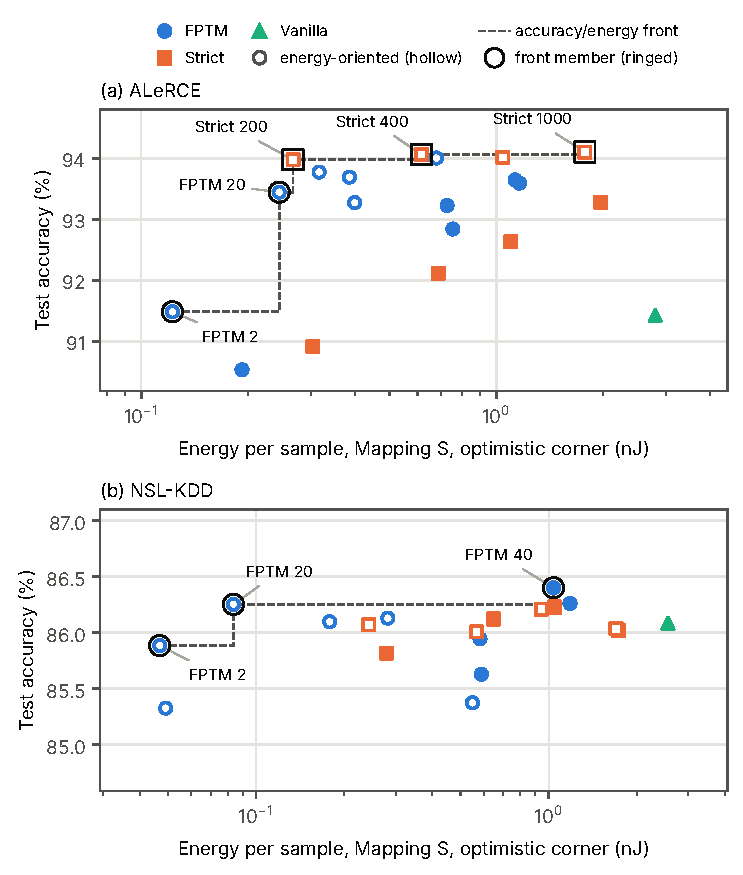
\includegraphics[width=0.92\textwidth]{figures/acc_energy_front.pdf}
\caption{\wosnew{Test accuracy versus Mapping~S energy per sample (optimistic corner) for the accuracy-oriented (filled) and energy-oriented (hollow) hyperparameters. The dashed line is the accuracy and energy front, and ringed points are its members. Unringed points near the line are dominated by less than 0.05 points. Energy includes the controller. The axes are cut to the front region. Below the cut lie the 200-clause vanilla TM of both datasets (78.65\% and 81.22\%) and the accuracy-oriented 2-clause NSL-KDD FPTM (84.11\%).}}
\label{fig:front}
\end{figure}

\paragraph{WOS-46985}\label{sec:wosretune}
\wosnew{On WOS-46985, the two runs differ by at most 0.61 points in accuracy and 32\% in energy.
The energy-oriented FPTM models carry 102 to 607 literals per clause, against 215 to 1,168 with the accuracy-oriented settings. Their energy falls by $2.6\times$ to $25\times$, and their accuracy rises by 0.96 to 3.01 points.
Part of this gain comes from the longer schedule. The 2-clause FPTM, for example, reaches its best validation accuracy only at epochs 239 and 274 of the two runs.}
\wosnew{Even so, the front holds strict models only: the accuracy-oriented and energy-oriented 200-clause models and the energy-oriented 400-clause model.
The cheapest FPTM has 10 clauses per class. It needs 21\% to 23\% more energy than the accuracy-oriented 200-clause strict model} (\hyp{3.77~nJ} and \hyp{1.11~nJ}, 90.87\%). \wosnew{It is also 2.04 points less accurate.
The energy-oriented 200-clause strict model has longer clauses (94 against 74 literals) and needs 13\% to 14\% more energy at the same cycle count.
WOS-46985 is thus the case where FPTM does not pay off on \gainp{}: its text clauses stay long, and long clauses need long miss counts.}
\section{Discussion}\label{sec:discussion}

\paragraph{When FPTM pays off on \gainp{}}
In software, FPTM saves memory and training time by needing fewer clauses~\cite{hnilov2025fptm}.
On an associative processor the cost model differs.
A strict clause of any length is one search \wosnew{cycle}, so the \wosnew{cycle count} of a strict model grows with its number of clauses. \wosnew{In Mapping~S, its energy also grows with the number of unmasked rows, i.e., with the clause length.}
A fuzzy clause needs a miss count, which a binary-sensed search cannot produce in one step.
Its cost grows with its number of literals. With the thermometer counter, each literal costs up to $3b_j$ cycles. With the binary counter, it costs about $5\log_2$ of the literal index.
FPTM therefore pays off on \gainp{} when its clause reduction outweighs the cost of counting.
\wosnew{With the accuracy-oriented hyperparameters, this holds on ALeRCE.} There, 20 FPTM clauses per class are more accurate than 600 strict clauses, at fewer cycles and lower energy.
The 40-clause FPTM is also slightly more accurate than the 1,000-clause strict model, at lower cost. \wosnew{The margin is 0.36 points against this single-seed baseline, or 0.15 points against its first-round variant (Section~S1 of the supplementary material).}
\wosnew{With the energy-oriented hyperparameters, the 200-clause strict model gains 3.06 points, and FPTM keeps only the low-energy end of the ALeRCE front.
On NSL-KDD, FPTM models form the whole front, led by the energy-oriented 2-clause and 20-clause models. With the accuracy-oriented ones, strict models were cheaper at moderate accuracy.
On WOS-46985, the FPTM clauses stay long even after tuning, and long clauses need long miss counts. Strict models remain cheaper there with both sets.}

\wosnew{\paragraph{Accuracy versus energy}
The two hyperparameter sets show that the \gainp{} cost of FPTM follows its total number of included literals and its miss tolerance, rather than its clause count alone. Section~S8 of the supplementary material quantifies this relation.
On ALeRCE, the 1,000-clause strict model gains 0.65 points over the 20-clause FPTM at $7.2\times$ the energy.
On NSL-KDD, the most accurate models differ by less than the 0.5-point resolution of the test set, but by more than $20\times$ in energy.
On these two datasets, a designer who accepts a small loss can choose a compact FPTM model and save most of the energy.
On WOS-46985, the compact choice is a strict model.
When FPTM targets an associative processor, the training should therefore aim at few included literals as well as at few clauses.}

\paragraph{Application perspective}
A TM rule base is readable whether its clauses are strict or fuzzy.
A fuzzy clause reads as a conjunction that tolerates a bounded number of failed conditions.
\wosnew{A rule base with fewer literals is easier for a domain expert to inspect, and on \gainp{} it is also cheaper.
On ALeRCE, the energy-oriented 20-clause FPTM has $4.4\times$ fewer literals than the 200-clause strict model, which is 0.53 points more accurate. On NSL-KDD, the energy-oriented 20-clause FPTM, with 8.8 literals per clause, is the cheaper rule base at the same accuracy, within the resolution of the test set. On WOS-46985, the strict rule base is cheaper.}
For alert classification, LSST expects several million alerts per night~\cite{ivezic2019lsst}. \hyp{Even 10 million alerts in an 8-hour night amount to about 350 alerts per second.
In Mapping~S, a macro of 256 subarrays holds 25 stacks of 10 subarrays, i.e., 1,600 ALeRCE samples. Its 250 occupied subarrays and its model SRAM occupy about 0.19~mm$^2$ at 7~nm. It would classify a batch with the 20-clause FPTM in about 0.41~ms at the conservative corner, including input loading. This corresponds to about $3.9\times10^6$ samples per second, about $11{,}000\times$ the average alert rate above.
The program takes the same time for a partly filled batch, so alerts need not wait for a full batch. The energy per sample then rises, because the controller energy is shared by fewer samples.}
This comparison covers only the classification step. Light-curve feature extraction and booleanization are not part of it.
For intrusion detection, Mapping~C classifies one record at a time with the input on the searchlines. \hyp{The 20-clause NSL-KDD FPTM needs about 6.9~$\mu$s per record at the conservative corner.} This latency covers the in-array part only. The external reduction of about 458 clause scores into class votes is not included. We do not compare this latency with a line-rate requirement. The features of NSL-KDD are computed per connection, and their extraction is not modelled.

\wosnew{Section~S9 of the supplementary material discusses the strict models of the FPTM trainer and the choice between the two mappings.}

\paragraph{Directions}
\hyp{Three directions follow from the cost structure.
(i) Multi-level sensing. In \gainp{}, mismatch readout is additive, and more mismatching cells shift the matchline voltage further from the match case~\cite{levi2026gainp}. A sense amplifier that resolves a few mismatch levels would turn the FPTM miss count into a single search and remove the main penalty of fuzzy clauses.
(ii) Inter-column reduction. A small adder tree at the subarray edge would make Mapping~C complete for both strict and fuzzy models.
(iii) Cost-aware training. The Mapping~S cycle count grows with the total literal count of the fuzzy clauses. A literal-count regularizer or a smaller $\LF$ could lower the \gainp{} cost of FPTM.}
Directions (i) and (ii) are not evaluated here. \wosnew{For (iii), the energy-oriented hyperparameters of Section~\ref{sec:energyhp} are a first step. Tuned for few included literals, they cut the FPTM energy by up to $3.7\times$ on ALeRCE, $12\times$ on NSL-KDD and $25\times$ on WOS-46985.}


\paragraph{Scope}
The 7~nm \gainp{} design has not been fabricated. The area of the sequencer logic and the area and energy of the prefetch buffer are not modelled (Section~\ref{sec:eval}).
The energy-oriented settings were chosen by hand on the validation split. Their results use two runs on ALeRCE and WOS-46985 and one run on NSL-KDD.
The 1,000-clause models and the WOS-46985 vanilla TM use one seed.

\section{Conclusions}\label{sec:conclusions}
\wosnew{We mapped Fuzzy-Pattern Tsetlin Machine inference onto \gainp{}, a GC-eDRAM associative in-memory processor, using only its compare, write and read primitives.
A sample-stationary and a clause-stationary layout were studied. Exact compile-time clause simplification and two in-array miss counters make the mapping practical.
For all 80 trained models of the main experiments and the 46 energy-oriented models, the in-array predictions matched a software reference on all checked test samples.}

\wosnew{The hardware evaluation targets a new 7~nm \gainp{} design.
A strict clause costs one search cycle regardless of its length, while a fuzzy clause costs a bit-serial miss count.
The \gainp{} cost of FPTM therefore follows its total number of included literals and its miss tolerance, rather than its clause count alone.
With the accuracy-oriented hyperparameters, FPTM pays off on ALeRCE. There, the 20-clause FPTM is more accurate than a 600-clause strict model and needs} \hyp{about $1.5\times$ less energy}. \wosnew{Strict models are cheaper on WOS-46985, and on NSL-KDD at moderate accuracy.
Energy-oriented hyperparameters, tuned for few included literals, cut the FPTM energy by up to $3.7\times$ on ALeRCE, $12\times$ on NSL-KDD and $25\times$ on WOS-46985.
On NSL-KDD, FPTM models then form the whole accuracy and energy front. In one run, a 20-clause FPTM reaches the accuracy of the most accurate strict model, within the 0.5-point resolution of this test set, at $12.9\times$ less energy.
On ALeRCE, FPTM gives the two cheapest points of the front, and strict models give the highest accuracy. On WOS-46985, strict models stay cheaper.
On all three datasets, the last fraction of a point of accuracy costs $2\times$ to more than $20\times$ in energy.
FPTM is therefore the better rule base on \gainp{} when its clauses stay short, as on ALeRCE and NSL-KDD, and the strict rule base when they stay long, as on WOS-46985.
In the clause-stationary layout, the accuracy-oriented 20-clause ALeRCE FPTM needs about $47\times$ less array area than the 1,000-clause strict model. It needs a longer latency and} \hyp{$1.6\times$ to $4.9\times$} \wosnew{more energy per sample.}

\hyp{In the sample-stationary layout, the \gainp{} energy per classification, excluding model-SRAM leakage, lies within the range reported for TM ASICs and in-memory designs. It is below that of TM FPGA accelerators. These designs use other datasets and models. Under a 1~W core-power bound, a single-thread CPU needs $63\times$ to about $7{,}100\times$ more energy for every model. For astronomical alert classification, one 0.19~mm$^2$ macro would classify about $11{,}000\times$ the average alert rate expected from LSST.}

\hyp{Multi-level matchline sensing, an inter-column reduction unit and cost-aware FPTM training are possible ways to remove the miss-count penalty of fuzzy clauses. Silicon characterization of the 7~nm \gainp{} will replace the modeled parameters.}

\section*{Data and code availability}
The FPTM reference implementation is publicly available at \url{https://github.com/BooBSD/FuzzyPatternTM}~\cite{hnilov2025code}. The datasets are publicly available from their original sources~\cite{kowsari2017hdltex,sanchezsaez2021alerce,tavallaee2009nslkdd}. The ALeRCE and NSL-KDD splits follow the published TreeTM preparation code~\cite{treetm2026repo}.

\section*{CRediT authorship contribution statement}
\textbf{Artem Hnilov:} Software, Data curation, Methodology, Validation, Formal analysis. \textbf{Alexander Fish:} Conceptualization, Visualization. \textbf{Leonid Yavits:} Conceptualization, Writing (original draft), Writing (review and editing), Supervision, Project administration, Resources.

\section*{Declaration of competing interest}
The authors declare that they have no known competing financial interests or personal relationships that could have appeared to influence the work reported in this paper.

\section*{Declaration of generative AI and AI-assisted technologies in the manuscript preparation process}
AI was used in preparation of this work.

\bibliographystyle{elsarticle-num}
\bibliography{refs}
\end{document}
